\section{АНАЛІЗ ФАКТОРІВ ВПЛИВУ}
Внаслідок розробки великої кількості нових рекомендаційних алгоритмів постало критичне питання у вітсутності єдиного підходу до оцінки їх еффективності, що призводитть до нерепродуктивних та несправедливих результів їх порівняння.

Також, побудова кожної системи рекомендацій складається із багатьох етапів які можна класифікувати на дві умові групи:
\begin{itemize}
    \item Фактори залежні від моделі
    \item Фактори не залежні від моделі
\end{itemize}
Кожен із них критично впливає на результат і залежить один від одного. Більше того їх оптимальні значення і характеристики не відомі. Тому важливо їх детально дослідити.

Фактори не залежні від моделі відповідають специфічним рішенням при пректуванні системи без прямого впливу на сам алгоритм і методів його оптимізації (тобто говоримо про вибір та підготовку навчальної вибірки, деталей проведення валідації).

Інші фактори, навпроти, включають у себе вибір таких речей як функція втрат, оптимізатор і метод регуляризації.
Розглядаючи типовий процес побудови рекомендацій варто виділити наступні  етапи:
\begin{enumerate}
    \item Вибір спліт методу (Dataset Spliting Method).
    \item Вибір метрики якості (Evaluation Metric Selection).
    \item Формулювання функції втрат для оптимізації (Loss function design).
    \item Методологія негативного семплінгу (Negative Samoling Strategy).
    \item Стратегія ініціалізації вагів (Parameter Initializer Selection).
    \item Вибір алгоритму оптимізації (Model Optimizer Selection).
    \item Вибір методу регуляризації (Regularization Term /  Dropout).
    \item Критерії останова (Early Stop Mechanism).
    \item Донавчання вагів (Hyper Params Tuning).
\end{enumerate}
Для кожного із вищевказаних факторів впливу відберемо кандидатів для експерементального дослідження. Нашою метою є пошук оптимального підходу до побудови ефективної моделі рекомендацій.
\begin{figure}
    \centering
    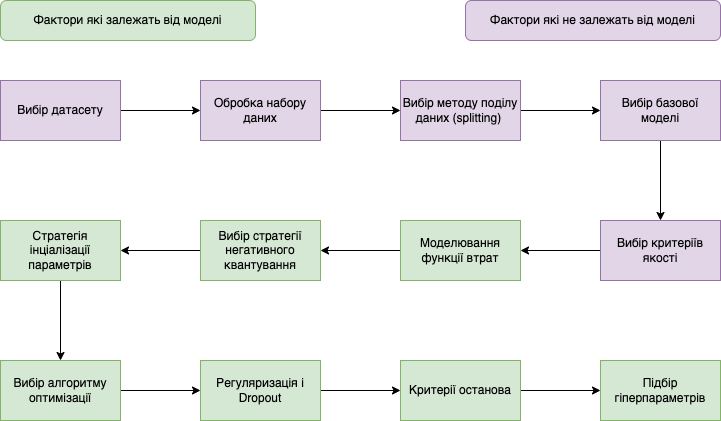
\includegraphics[width=0.9\textwidth]{images/FactorsTypes.png}
    \caption{Розглянутий пайплайн із поділом факторів впливу на категорії}
\end{figure}
\subsection{Вибір спліт методу}
Розглянувши набори даних які використовують для побудови рекомендацій, потрібно звернути увагу на розділ датасету на навчальну вибірку і вибірки для тестування (валідації). Валідація виконується для упередження перенавчання моделі, тобто алгоритм перестає широко генералізовуватись і починає змінювати ваги виключно під навчальні екземпляри. Після падіння метрик якості протягом 3-10 епох потрібно зупинити навчання і перейти до тестування на фільній вибірці.

Вибір спліт методу залежить від структури даних, а саме від присутності у них відмітки про час виконання дії. Що, надає можливість обрати одну із двох стратегій поділу.

У класичному підході в задачах машинного навчання, ми вважаємо що кожен зразок навчальної вибірки є не залежним один від одного. І не розглядаємо ймовірність коваріацій між взаємодіями одного користувача у розрізі часу (час взаємодій не впливає на використання). У цьому випадку використовують так званий поділ за співвідношенням. Тобто, ми ділимо датасет на групи відносно деякої пропорції, зазвичай $80\%$ на $20\%$, $80\%$ відходить на навчальну вибірку (разом із валідацією), а $20\%$ на тестування.

Другий можливий підхід - це поділ відносно часу. У навчальній вибірці беруть k спостережень певного користувача із максимальним timestamp (відміткою часу) t, а у тестовий набір попадають наступні n екземплярів із  timestamp більше t.
Тобто ми перевіряємо здатність моделі передбачити n наступних взаємодій.
\subsection{Підготовка даних}

\textbf{Для тестового набору}. Для завдання побудови рекомендацій потрібно зберігати повноту вибірки для тестування відносно користувачів. Що значить, що для кожного користувача який попадає у даний набір потрібно зберігати одинакову кількість його спостережень (наприклад не менше 5 оцінок на 1 унікальний user\_id).
У таблиці 7.1 наведено розраховані розміри вибірок для кожного користувача.
\begin{table}[]
    \centering
    \caption{Середня кількість екземплярів для кожного унікального користувача}
    \begin{tabular}{|c|c|c|c|}
        \hline
        Тип        & ML-1M & LastFm & Netflix \\ \hline
        Навчальний & 86    & 39     & 161     \\ \hline
        Тест       & 64    & 10     & 84      \\ \hline
    \end{tabular}
    \label{tab:size_of_split}
\end{table}

\textbf{Для тренувального набору}. Дані проходять додаткову фільтрацію від неактивних користувачів. Усі користувачі кількість взаємодій яких менше порогового значення видаляються із навчальної вибірки. Розглядаємо такі порогові значення [без фільтрації, 5, 10] 


\subsection{Вибір метрики оцінки якості}
Із великого різноманіття розглянутих метрик, було обрано шість основних метрик: Precision@k, Recall@k, MAP, HitRatio,  Mean Reciprocal Rank, NDCG. 
Для метрик які оцінюють фактичну присутність релевантних обєктів у рекомендаціях (*.@k) розглядаємо k у інтеравалі між [10,50].
\begin{figure}[H]
    \centering
    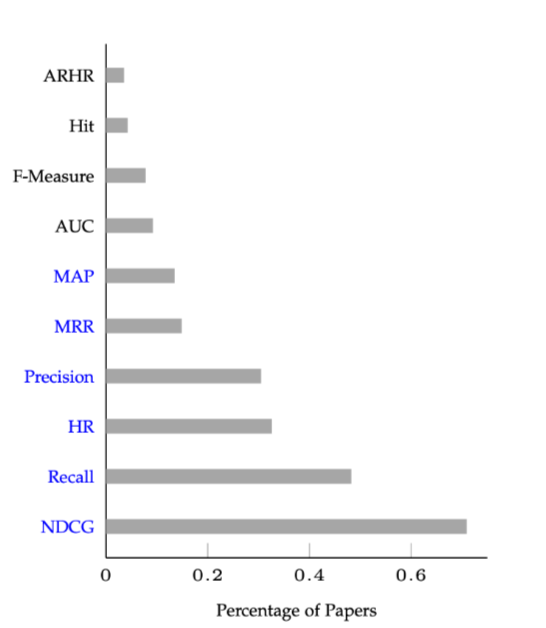
\includegraphics[width=0.6\textwidth]{images/metric_hist_papers.png}
    \caption{Розподіл використання метрик у наукових статтях}
\end{figure}

Метрики оцінюють передбачування моделей із точки зору класифікації і ранжування. Додатково потребує оцінка значень метрик різноманітності. Формулювання яких наведено у Розділі 4. 

\subsection{Стратегії негативного семплювання}
Вибірка об’єктів рекомендацій часто досягає надзвичайно великих розмірів.
Так, як моделі на виході повертають оцінку релевантності для цих об’єктів, на 
кожній ітерації навчання потрібно обновлювати ваги і розраховувати передбачення для кожного елементу. Що є не ефективно із точки зору вартості обчислень. Додатково, більшість користувачів знайомі лише із малою вибіркою елементів. Тому відсутність оцінки/взаємодії може вказувати не на низьку релевантність, а на те що об’єкт їм не відомий.

Для вирішення цієї проблеми використовують негативний семплінг. 

Його ідея полягає у відборі певної групи елементів, які не оцінені користувачем в минулому. 

В літературі розглядають декілька варіантів семплювання: із нормального розподілу, семплювання на основі низької популярності і семплювання із елементів високої популярності.

\begin{itemize}
    \item \textbf{Семплювання із нормального розподілу}. Обираємо n об’єктів керуючись їх ймовірністю.
    \item \textbf{High popularity sampling}.На основі розрахованих оцінок популярності обираємо top n кандидатів. Відсутність оцінки у невідомого,але популярного об’єкта явно вказує на низьку релевантність для користувача, порівняно із випадковим кандидатом.
    \item \textbf{Low popularity sampling}. Співпадає із high popularity, але вибираємо елементи із хвоста.
    \item Комбінування обох підходів.
\end{itemize}

\subsection{Стратегії ініціалізації параметрів}

Зазвичай у моделях побудови рекомендацій присутній набір параметрів, оптимізація яких навчає алгоритм. Їх вид залежить від обраної архітектури моделі і може бути як матрицею взаємодій, так і вагами нейромереж.
Привильний підхід до їх ініціалізації приводить до скорішого навчання і сходимості. Для моделей які будують приховане відображення взаємодій (латентні фактори) типовим є використання рівномірного $\mathcal{U}(0, a)$ і нормального $\mathcal{N}(0, \sigma^{2})$ розподілів, із значеннями $a = 1$ і $\sigma = 0.01$ відповідно.

Нейромережі особливо чутливі до початкових значень вагів. При не оптимальному підході, функція втрат змінюватись не буде, навіть після декількох десятків епох. Занадто малі значення приводять до затухання, коли функції активацій у нейронах залишаються неактивними (навіть у випадку використання таких функцій як LeakyReLU). Великі значення, навпроти, приведуть до зривних градієнтів.

У завданнях побудови рекомендацій із допомогою нейронних мереж використовують метод ініціалізації Ксавєра:
\[ W_{ij} \sim \mathcal{U}(- \frac{1}{\sqrt{n_{in} + n_{out}}}, \frac{1}{\sqrt{n_{in} + n_{out}}}) \]

Де $W_{ij}$  матриці вагів нейромереж, $n_{in}$, $n_{out}$ розмір вхідного і вихідного шару.

\subsection{Вибір методу оптимізації моделей}

\begin{figure}
    \centering
    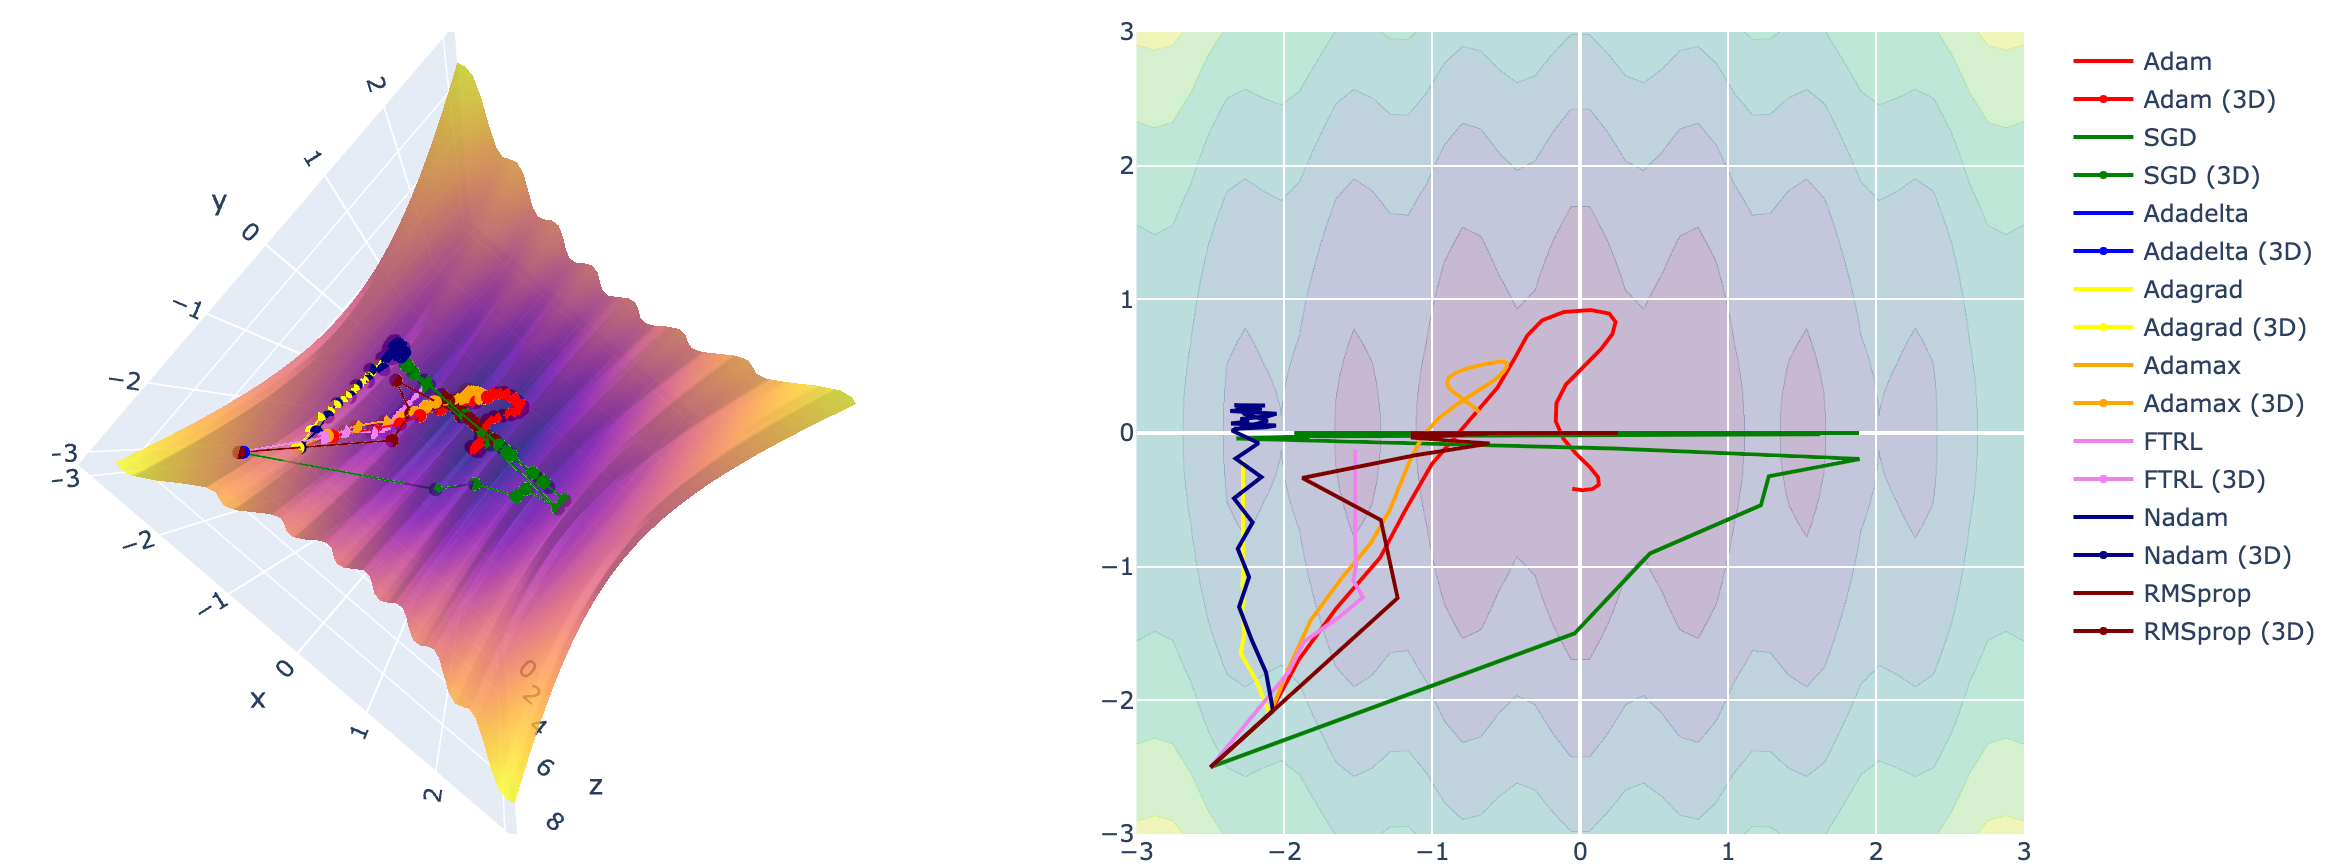
\includegraphics[width=0.9\textwidth]{images/sgd.png}
    \caption{Результат роботи різних варіантів градієнтного спуску}
\end{figure}

Оптимізатор використовується для оновлення параметрів моделі, мінімізуючи функцію втрат у пошуках глобального мінімуму. Різні оптимізатори впливають на роботу алгоритмів рекомендацій.

\textbf{Градієнтний спуск}.
Один із найпопулярніших ітераційних методів оптимізації першого порядку, основа багатьох наступних його варіацій. Розглядається задача пошуку локального мінімуму деякої функції $\mathcal{L}: \mathbb{R}^{n} \rightarrow \mathbb{R}$:
\[\mathcal{L} \rightarrow \min_{\theta \in \mathbb{R}^{n}}  \]
Ідея методу полягає в тому, щоб виконати оптимізацію в напрямку найшвидшого спуску, який задається антиградієнтом  $-\nabla_{\theta} f$:
\[\theta_{t+1} = \theta_{t} - \lambda  \nabla_{\theta} \mathcal{L}(\theta_t) \]
де $\lambda$ обирається одним із декількох варіантів:
\begin{itemize}
    \item Константа, у цьому випадку метод може не зійтись.
    \item Дробовим кроком, який змінюється.
    \item Найшвидшим cпуском : $\lambda_t = \arg \min_{\lambda} \mathcal{L} (\theta_t) - \lambda \nabla_{\theta} \mathcal{L}(\theta_t) $.
\end{itemize} 
Критерій останова для градієнтного спуску:
\[|\mathcal{L}(\theta_{t+1}) -  \mathcal{L}(\theta_t)| < \epsilon\]
де $\epsilon$ наперед задане невідємне число.

\textbf{Стохастичний градієнтний спуск}.Коли алгоритм проходить через навчальний набір, він виконує вищезазначене оновлення для кожного елемента датасету. Виконуючи перетасування, можна виконувати декілька проходів до збіжності, вибираючи оптимальний крок $\lambda$.

\[\theta_{t+1} = \theta_{t} - \lambda  \nabla_{\theta} \mathcal{L}(\theta_t, (u,i)) \]

\textbf{Пакетний градієнтний спуск}. Результат подальшого розвитку градієнтного спуску. В результаті експериментів було виявлено ефективність обновлення вагів сумою групи (пакету) елементів. Тобто, на одній ітерації значення вагів акумулюються і оновлюється їх сумою. Що прискорює збігання

\[\theta_{t+1} = \theta_{t} - \lambda  \nabla_{\theta} \mathcal{L}(\theta_t, B(u,i)) \]

\textbf{Адаптивний градієнт AdaGrad}. У завданнях обробки мови, фільтрації спаму чи побудови рекомендацій вхідний сигнал, тобто дані, часто бувають розріджені (У наших датасетах, наприклад Sparsity 99.99+\%). Така ситуація приводить до того що інформативні признаки зустрічатимуться достатньо рідко, і із іншої сторони, глобальні шаблони будуть зустрічатись надзвичайно часто (більшість користувачів знайомі із фільмами Володар Перстнів). Тому, було б зручно, визначати наскільки деякий признак часто зустрічається у навчальній вибірці, або як часто він приводить до активації нейронів. Ідея вирішення достатньо проста - ми будемо зберігати для кожного параметру мережі частоту його обновлення. І у випадку коли параметр навчається повільно (частота обновлень низька) ми будемо збільшувати його вплив.  
\[ \theta_{t + 1} = \theta_t - \frac{\lambda}{\sqrt{G_t + \eta}} \cdot \nabla_{\theta}\mathcal{L}(\theta_t)\]
де $G_t$ відповідає за частоту оновлення, а $\eta$ є деякий ненульовий фактор щоб вберегти ділення на 0. У параметра який часто обновлюється, великий $G_t$, і його вплив штрафується. Додатково, метод не сильно чутливий до вибору $\lambda$, достатньо обрати його один раз.
\newpage
\textbf{RMSProp}. Адаптивний градієнт має властивість затухати при великих значеннях $G_t$. Модифікацію, що вирішує проблему паралічу алгоритму називають RMSProp. 
\[ \theta_{t + 1} = \theta_t - \frac{\lambda}{\sqrt{\mathbb{E}[g^{2}_t] + \eta}} \cdot \nabla_{\theta}\mathcal{L}(\theta_t)
\]
Ми все ще збираємось оновлювати ваги, які занадто часто оновлюються, але замість повної кількості оновлень ми будемо використовувати квадрат  середнього градієнту в історії. Ми використовуємо експоненціальне згасаюче середнє $\mathbb{E}[g^2]$:
\[\mathbb{E}(g^{2})_t = \gamma \mathbb{E}[g^{2}]_{t-1}+ (1 - \gamma)g^{2}_t\]
% \subsection{Регуляризація}
\subsection{Критерії останова та Регуляризація}
\begin{figure}
    \centering
    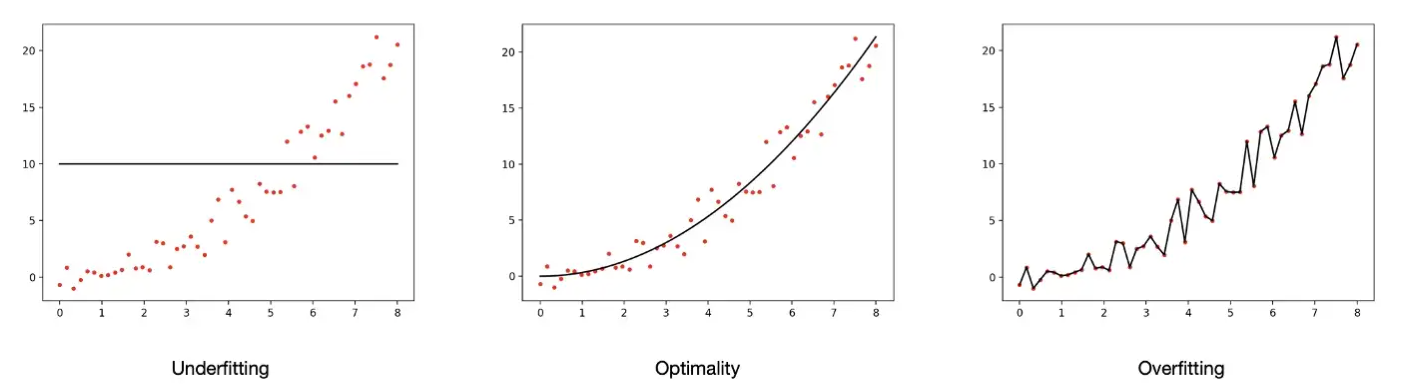
\includegraphics[width=1\textwidth]{images/fiting_problems.png}
    \caption{Приклад недонавчання, перенавчання і оптимального стану функцій втрат}
\end{figure}
У машинному навчанні використовуються різні стратегії для боротьби з проблемою перенавчання, яка приводить до гіршої генералізації, тим самим досягаючи низької ефективності на тестувальній вибірці (Рис. 6.4). Власне, найбільш широко використовувані методи регуляризації включають регуляризацію, механізм dropout та раньої зупинки.

\textbf{Регуляризація}. Як правило, фактор інтегрується в функцію втрат, щоб допомогти уникнути перенавчання під час навчання моделі рекомендації. В основному використовують два види, а саме регуляризація L1 та L2 (які також відомі як норми). Норма L1 відома як Манхетенська відстань, яка є найбільш природним способом вимірювання відстані між векторами. Це сума величин векторів у просторі, де всі компоненти вектора зважуються однаково. Норма L2 є найпопулярнішою нормою, також відомою як евклідова норма, відповідає  найкоротшій відстані між двома точками. 
Головними відмінностями у використані цих двох норм: L1 регуляризація намагається оцінити медіану даних, коли L2 оцінює середнє.
Додатково L1 норма виконує функцію feature selection -  відбирає лише важливі признаки, що корисно, враховуючи велику кількість признаків у завданнях Глибокого навчання.

\begin{figure}
    \centering
    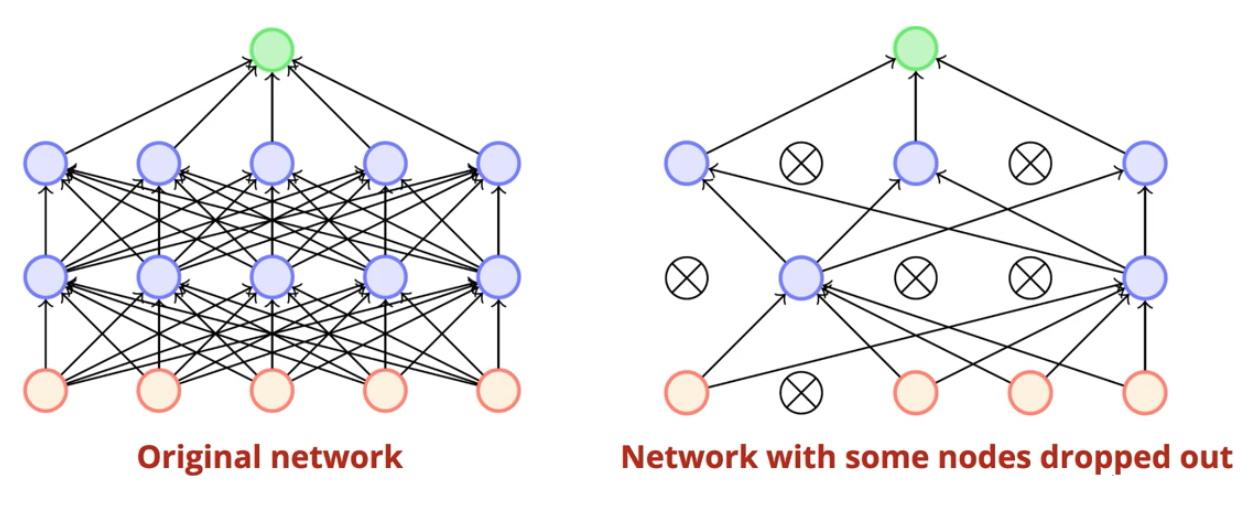
\includegraphics[width=1\textwidth]{images/dropout.png}
    \caption{У результаті Dropout, кожен нейрон із деякою ймовірністю може бути ”виключеним”}
\end{figure}
\textbf{Dropout}. Широко прийнятий у Глибокому навчанні метод, для упередження перенавчання. Ключова ідея полягає в тому, щоб випадковим чином відключити нейрони (разом із їх зв’язками) із мережі під час тренувань, що заважає мереді занадто сильно адаптуватись (Рис 6.5) . Отже, вводиться додатковий гіперпараметр, тобто ймовірність збереження нейрона Р, для контролю інтенсивності виключення. Типові значення P для нейронів прихованих шарів  знаходяться в діапазоні від 0,5 до 0,8.

\textbf{Механізм ранньої зупинки}. Рання зупинка - це також форма регулізації, яка використовується для уникнення надмірного перенавчання. Основна проблема моделей побудови рекомендацій(наприклад, LFMS та DLM) полягає у виборі кількості навчальних епох. Занадто багато епох можуть призвести до надмірної підстановки вагів до навчального набору даних, тоді як занадто мало може призвести до слабкої моделі. Рання зупинка - це метод, який дозволяє нам вказати довільну велику кількість навчальних епох і припинити навчання, як тільки  продуктивність моделі перестає вдосконалюватись на валідаційному наборі протягом декількох епох.
\subsection{Підбір гіперпараметрів}
Кожен гіперпараметр заданий набором можливих значень (тобто простором пошуку) на основі емпіричного знання, а оптимальне налаштування отримується шляхом проходженням через увесь простор пошуку. Такий підхід називається Grid Search. Основним його недоліком є обчислювальна нефективність, а у випадку великої кількості гіперпараметрів, його використання не доцільне. Припустимо, модель має m гіперпараметрів, де кожен параметр має у середньому n можливих значень, модель потрібно навчати NM разів, щоб знайти оптимальні значення для всіх гіперпараметрів.

RandomSearch, використовує одинакой піхід, тільки простір можливих значень вибирається випадково. 

Одним із більш оптимальних підходів, є так званий Bayesian HyperOpt.
Підхід байєсівської оптимізації фокусується на моделі ймовірності $P(score| configuration)$, яка оновлюється через ітеративний процес завдання якого є максимізація оцінки, враховуючи конфігурацію "C”. Hyperopt приймає байєсівську оптимізацію як свою передумову, зробивши деякі варіації в процесі вибірки, визначення та звуження простору пошуку та алгоритмів для максимізації моделі ймовірності.
\subsection*{Висновки}

У розділі розглянуто широкий набір фаторів впливу на якість моделей побудови рекомендацій. Представлено їх поділ відносно характеру впливу. Проаналізовано природу факторів, запропоновані варіації факторів для експериментального дослідження.